\documentclass[conference]{IEEEtran}
\usepackage{cite}
\usepackage{amsmath,amssymb,amsfonts}
\usepackage{algorithmic}
\usepackage{graphicx}
\usepackage{textcomp}
\usepackage{xcolor}
\usepackage{tikz}
\usetikzlibrary{shapes.geometric, arrows, positioning}
\usepackage[hidelinks]{hyperref}

\begin{document}

\title{``MultiModalQA-Agent'': A Multimodal LLM Agent for Question Answering over Text and Images using MCP}

\author{
\IEEEauthorblockN{Paul Odimmegwa}
\IEEEauthorblockA{\textit{Department of Computer Engineering} \\
\textit{Warsaw Management University}\\
Student ID: 78687}
\and
\IEEEauthorblockN{Takura Lionel Muparutsa}
\IEEEauthorblockA{\textit{Department of Computer Engineering} \\
\textit{Warsaw Management University}\\
Student ID: 79215}
\and
\IEEEauthorblockN{Haytham Dyabi}
\IEEEauthorblockA{\textit{Department of Computer Engineering} \\
\textit{Warsaw Management University}\\
Student ID: 78247}
\and
\IEEEauthorblockN{Erlanbek Arapbaev}
\IEEEauthorblockA{\textit{Department of Computer Engineering} \\
\textit{Warsaw Management University}\\
Student ID: 79083}
\and
\IEEEauthorblockN{Mr. Kumar Nalinaksh}
\IEEEauthorblockA{\textit{Professor} \\
\textit{Warsaw Management University}\\
kumar.nalinaksh@office.mans.org.pl                                                                                              }
}

\maketitle


\begin{abstract}
LLMs have drastically increased language understanding and answering question systems. But, lots of current systems are very limited to process data that are just textual, this make them untrustworthy in cases like distributing context in both text and images. In knowledgeable materials, diagrams, screenshots, lecture slides and many more often showcase visuals rather than textual. This brings challenges for text-only systems. We present MultiModalQA-Agent, a multi agent design to answer questions with both visual answers and textual answers. The system cooperates Retrieval-Augmented Generation, Model Context Protocol and LLMs tools to apprehend information sources. The system interprets textual and visual information from images and gets important textual context and generates grounded answers in multimodal. Also, the help from architecture when image information or textual information is not complete.
\end{abstract}

\begin{IEEEkeywords}
Multimodal LLMs, Answering Questions, Vision-Language Models, Multi-Agent Systems, MCP, Understanding Image, Retrieval-Augmented Generation 
\end{IEEEkeywords}

\section{Introduction}
The increasing development of LLMs has changed the knowledge of language processing, summarizing documents, and question answering. Regardless of these accomplishments, many AI assistants work solely on textual data and are limited in their ability to reason over visual information. In practical scenarios, users frequently collaborate with mixed content such as diagrams, annotations, and screenshots. Text-based systems often miss the mark when trying to interpret the full meaning of these multimodal content. To address these restrictions, we suggest MultimodalQA-Agent, a forced multi-agent framework that makes use of MCP-based coordination to organize multiple precision tools.

\section{Literature Review}
\subsection{Multimodal Large Language Models}
Multimodal Large Language Models expand LLM abilities by integrating language reasoning and vision. Models like GPT-4 Vision and CLIP show powerful capabilities in image captioning and visual understanding.

\subsection{Multi-Agent Systems}
Multi-agent structures separate difficult assignments into subgroups maintained by dedicated agents. While systems like AutoGen show how structured agents can organize tool usage, they rarely integrate multimodal reasoning with organized orchestration rules like MCP.

\subsection{Retrieval Augmented Generation (RAG)}
RAG improves LLM performance by adding external knowledge retrieval prior to generation. While highly effective in reducing hallucinations, many RAG systems primarily concentrate on textual data and do not integrate image processing pipelines.

\subsection{Multimodal Evaluation}
Analyzing multimodal systems remains difficult as answers depend on both visual reasoning and textual understanding. Normal NLP metrics like ROUGE and BLEU do not capture multimodal understanding standards.

\subsection{Model Context Protocol (MCP)}
MCP allows organized communication between outside tools and language models, enabling agents to authorize expert features like OCR engines and image analyzers through uniform links.

\subsection{Summary and Research Gap}
Recent research shows progress in multimodal understanding and agent architectures, yet there is a limited structure that combines multi-agent coordination, uniform tool orchestration via MCP, and grounded multimodal grounding for tool orchestration and retrieval. This inspires the development of MultiModalQA-Agent.

\section{Challenges}
The following restraints are recognized in recent multimodal question-answering systems:
\begin{itemize}
    \item \textbf{Poor Robustness:} Systems fail when a single modality is incomplete.
    \item \textbf{Monolithic Architectures:} Lack of modular plans and adaptable tool arrangements.
    \item \textbf{Weak Explainability:} Users cannot see how answers were produced across modalities.
    \item \textbf{Hallucination Issue:} Models produce baseless explanations of visual data.
    \item \textbf{Limited Integration:} Processing images and text individually without cross-modal reasoning.
\end{itemize}

\section{Proposed Solution}
To address the limitations of existing text-only question-answering systems, we propose MultiModalQA-Agent, a multimodal intelligent assistant capable of understanding and reasoning over both text and images.

\subsection{Overall System Architecture}
The system processes multimodal inputs through a sequence of coordinated agents, as illustrated in Fig. \ref{fig:arch}.

\begin{figure}[htbp]
\centering
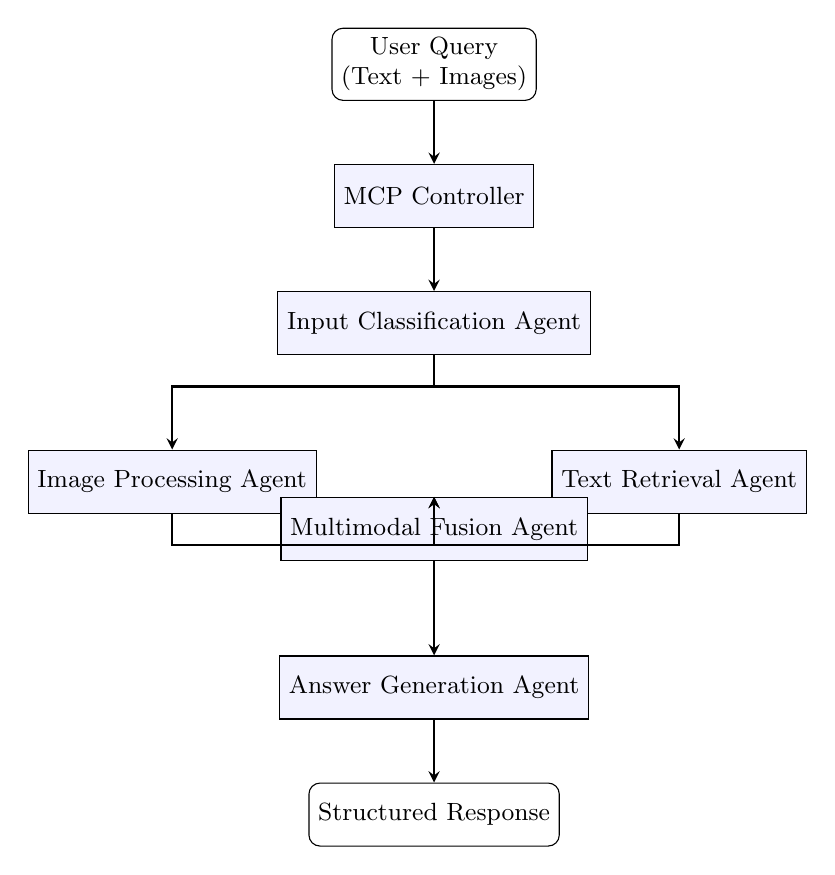
\begin{tikzpicture}[
    node distance=1.2cm,
    every node/.style={font=\small},
    box/.style={rectangle, draw, rounded corners, minimum width=2.5cm, minimum height=0.8cm, align=center},
    process/.style={rectangle, draw, minimum width=2.5cm, minimum height=0.8cm, align=center, fill=blue!5},
    arrow/.style={->, >=stealth, thick}
]
\node (input) [box] {User Query \\ (Text + Images)};
\node (mcp) [process, below=0.8cm of input] {MCP Controller};
\node (class) [process, below=0.8cm of mcp] {Input Classification Agent};
\node (img) [process, below left=1.2cm and -0.5cm of class] {Image Processing Agent};
\node (txt) [process, below right=1.2cm and -0.5cm of class] {Text Retrieval Agent};
\node (fusion) [process, below=1.8cm of class] {Multimodal Fusion Agent};
\node (gen) [process, below=1.2cm of fusion] {Answer Generation Agent};
\node (output) [box, below=0.8cm of gen] {Structured Response};
\draw [arrow] (input) -- (mcp); \draw [arrow] (mcp) -- (class);
\draw [arrow] (class.south) -- ++(0,-0.4) -| (img.north);
\draw [arrow] (class.south) -- ++(0,-0.4) -| (txt.north);
\draw [arrow] (img.south) |- ++(0,-0.4) -| (fusion.north);
\draw [arrow] (txt.south) |- ++(0,-0.4) -| (fusion.north);
\draw [arrow] (fusion) -- (gen); \draw [arrow] (gen) -- (output);
\end{tikzpicture}
\caption{Architecture of the MultiModalQA-Agent Framework.}
\label{fig:arch}
\end{figure}

\subsection{Core Components of the Framework}

\subsubsection{MCP Controller}
The MCP Controller acts as the central coordinator of the system. It determines:
\begin{itemize}
    \item Which tools should be activated,
    \item Which agents should process the input,
    \item How outputs are transferred between modules.
\end{itemize}
This orchestration mechanism enables dynamic and efficient workflow execution.

\subsubsection{Input Classification Agent}
This agent determines the nature of the user request:
\begin{itemize}
    \item Text-only,
    \item Image-only,
    \item Combined multimodal query.
\end{itemize}
The classification step allows the system to activate only the required tools, reducing unnecessary computation.

\subsubsection{Image Processing Agent}
The Image Processing Agent handles the interpretation and analysis of visual inputs. Its primary responsibilities include:
\begin{itemize}
    \item Diagram interpretation,
    \item Screenshot understanding,
    \item Visual feature extraction,
    \item Image-text localization.
\end{itemize}
The agent converts visual content into structured semantic representations that can be processed by subsequent modules.

\begin{table}[htbp]
\centering
\caption{Key Functions of the Image Processing Agent}
\label{tab:image_functions}
\begin{tabular}{|l|l|}
\hline
\textbf{Function} & \textbf{Description} \\ \hline
OCR Extraction & Extracts embedded text \\ \hline
Feature Detection & Identifies shapes and structures \\ \hline
Object Recognition & Detects visual components \\ \hline
Layout Analysis & Understands spatial relationships \\ \hline
\end{tabular}
\end{table}


\subsubsection{Text Retrieval Agent}
The Text Retrieval Agent performs semantic retrieval using vector similarity search to ensure that generated responses are backed by factual evidence. The agent:
\begin{itemize}
    \item Converts queries into high-dimensional embeddings,
    \item Searches vector databases for relevant context,
    \item Retrieves contextually relevant information to support answer generation.
\end{itemize}
This mechanism significantly improves factual grounding and reduces the likelihood of hallucinated responses.


\subsubsection{Multimodal Fusion Agent}
The Multimodal Fusion Agent is responsible for synthesizing information from diverse sources. It combines:
\begin{itemize}
    \item Visual embeddings from the image processing stage,
    \item OCR-extracted text and diagram annotations,
    \item Retrieved semantic context from external knowledge bases.
\end{itemize}
The fusion process aligns information from multiple modalities into a unified representation to facilitate complex reasoning.

\subsubsection{Reasoning and Answer Generation Agent}
This final agent performs high-level synthesis to produce the user response. It is responsible for:
\begin{itemize}
    \item Contextual reasoning across modalities,
    \item Summarization of retrieved and extracted data,
    \item Explanation generation for diagrammatic content,
    \item Final answer synthesis.
\end{itemize}
The output is generated in a structured and explainable manner, ensuring that the user understands the basis of the provided answer.


\begin{table}[htbp]
\centering
\caption{Design Objectives of MultiModalQA-Agent}
\label{tab:objectives}
\begin{tabular}{|l|l|}
\hline
\textbf{Objective} & \textbf{Description} \\ \hline
Multimodal Understanding & Process both text and images \\ \hline
Explainability & Provide transparent reasoning \\ \hline
Robustness & Handle incomplete inputs \\ \hline
Scalability & Support modular expansion \\ \hline
Accuracy & Improve contextual understanding \\ \hline
Grounding & Reduce hallucinated responses \\ \hline
\end{tabular}
\end{table}


\begin{table}[htbp]
\centering
\caption{System Workflow Operations}
\label{tab:workflow}
\begin{tabular}{|l|l|l|}
\hline
\textbf{Step} & \textbf{Operation} & \textbf{Responsible Agent} \\ \hline
1 & Receive user input & MCP Controller \\ \hline
2 & Detect input modality & Classification Agent \\ \hline
3 & Extract image information & Image Processing Agent \\ \hline
4 & Retrieve supporting text & Retrieval Agent \\ \hline
5 & Merge multimodal context & Fusion Agent \\ \hline
6 & Generate grounded answer & Reasoning Agent \\ \hline
7 & Return explainable response & Output Module \\ \hline
\end{tabular}
\end{table}

\section{Implementation}
The implementation of MultiModalQA-Agent focuses on integrating multimodal AI technologies within an MCP-controlled multi-agent environment. The framework is developed using Python and leverages modern AI libraries for specialized tasks including image understanding, semantic retrieval, and natural language generation.

\subsection{Technology Stack}
The framework is implemented using a robust stack of modern AI and web technologies, as summarized in Table \ref{tab:tech_stack}.

\begin{table}[htbp]
\centering
\caption{Implementation Technology Stack}
\label{tab:tech_stack}
\begin{tabular}{|l|l|}
\hline
\textbf{Layer} & \textbf{Technology} \\ \hline
Programming Language & Python \\ \hline
API Framework & FastAPI \\ \hline
LLM Engine & GPT-4 / LLaVA \\ \hline
Vision Processing & OpenCV \\ \hline
OCR Tool & Tesseract OCR \\ \hline
Embedding Model & SentenceTransformers \\ \hline
Vector Database & FAISS \\ \hline
Frontend Interface & Streamlit \\ \hline
Orchestration Layer & MCP \\ \hline
\end{tabular}
\end{table}

\subsection{Input Handling}
The system is designed to be highly versatile in accepting various document types. Supported inputs include:
\begin{itemize}
    \item Uploaded images and diagrams,
    \item High-resolution screenshots,
    \item PDFs and technical manuals,
    \item Plain text documents,
    \item Natural language user questions.
\end{itemize}
Supported image formats for visual processing include PNG, JPG, JPEG, and PDF-based screenshots.

\subsection{Image Processing Pipeline}
The visual analysis pipeline consists of multiple stages designed to transform raw pixels into semantic data.

\subsubsection{Image Preprocessing}
Input images are first enhanced to improve readability and extraction accuracy using techniques such as:
\begin{itemize}
    \item Noise reduction,
    \item Contrast enhancement,
    \item Grayscale conversion,
    \item Edge detection.
\end{itemize}

\subsubsection{OCR Extraction}
The OCR engine extracts textual data from visual layouts, specifically targeting:
\begin{itemize}
    \item Paragraphs and body text,
    \item Labels and titles,
    \item Captions and diagram annotations.
\end{itemize}

\subsubsection{Feature Encoding}
Visual information is converted into embeddings for semantic alignment. For example, a network architecture diagram is encoded into its structural relationships, component labels, and visual dependencies.

\subsection{Retrieval-Augmented Generation Pipeline}
The retrieval subsystem enables the model to access external knowledge and grounded information. The retrieval workflow operates as illustrated in Fig. \ref{fig:rag_flow}.

\begin{figure}[htbp]
\centering
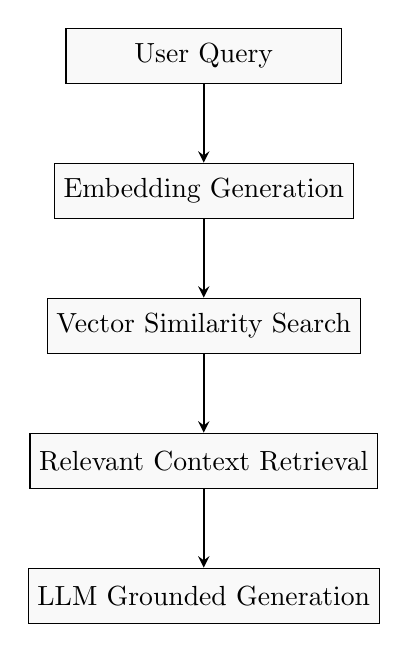
\begin{tikzpicture}[
    node distance=1cm,
    step_box/.style={rectangle, draw, minimum width=3.5cm, minimum height=0.7cm, align=center, fill=gray!5},
    arrow/.style={->, >=stealth, thick}
]
\node (query) [step_box] {User Query};
\node (emb) [step_box, below=of query] {Embedding Generation};
\node (search) [step_box, below=of emb] {Vector Similarity Search};
\node (context) [step_box, below=of search] {Relevant Context Retrieval};
\node (gen) [step_box, below=of context] {LLM Grounded Generation};

\draw [arrow] (query) -- (emb);
\draw [arrow] (emb) -- (search);
\draw [arrow] (search) -- (context);
\draw [arrow] (context) -- (gen);
\end{tikzpicture}
\caption{Retrieval-Augmented Generation (RAG) Workflow.}
\label{fig:rag_flow}
\end{figure}

The vector database serves as the long-term memory for the system, storing:
\begin{itemize}
    \item OCR outputs from previously processed images,
    \item User notes and annotations,
    \item Educational content and lecture materials,
    \item Knowledge-intensive technical documents.
\end{itemize}

\subsection{Multimodal Reasoning Mechanism}
The reasoning stage is where the system synthesizes diverse inputs to form a coherent understanding. The mechanism combines:
\begin{itemize}
    \item The original user question,
    \item Encoded visual context from images,
    \item Retrieved factual knowledge from the RAG pipeline,
    \item Raw OCR-extracted text and annotations.
\end{itemize}
The system performs semantic alignment across these sources before generating the final answer. For example, if an image contains a flowchart with technical labels and supporting text, the reasoning agent evaluates the relationships between these elements to produce a grounded explanation.

\subsection{Explainable Response Generation}
Unlike traditional black-box AI systems, the MultiModalQA-Agent framework is designed to provide transparent and explainable outputs. The final generated response typically includes:
\begin{itemize}
    \item Detailed diagram and visual interpretation,
    \item A concise summary of relevant textual information,
    \item Direct references to supporting evidence,
    \item Citations or links to retrieved context used in the reasoning process.
\end{itemize}

\subsection{Internal Communication Through MCP}
The Model Context Protocol (MCP) serves as the backbone for structured communication between autonomous agents. Table \ref{tab:mcp_functions} details how MCP facilitates the workflow.

\begin{table}[htbp]
\centering
\caption{MCP Internal Communication Functions}
\label{tab:mcp_functions}
\begin{tabular}{|l|l|}
\hline
\textbf{MCP Function} & \textbf{Purpose} \\ \hline
Tool Invocation & Activates required processing tools \\ \hline
Data Transfer & Passes outputs between specialized agents \\ \hline
Context Management & Maintains system-wide workflow state \\ \hline
Error Handling & Detects and recovers from processing failures \\ \hline
\end{tabular}
\end{table}

\subsection{Scalability and Extensibility}
The modular, agentic nature of the framework ensures it is highly extensible. Future iterations can integrate:
\begin{itemize}
    \item Audio processing agents for voice-based queries,
    \item Video understanding modules for temporal data analysis,
    \item Real-time collaboration tools for multi-user environments,
    \item Multilingual reasoning systems for global accessibility.
\end{itemize}

\section{Results}
The evaluation of MultiModalQA-Agent aims to measure the effectiveness of multimodal reasoning and MCP-based orchestration in complex question-answering tasks.

\subsection{Evaluation Setup}
The system was tested using a diverse range of materials to ensure robustness across different visual formats. The testing data included:
\begin{itemize}
    \item Educational lecture slides with mixed text and diagrams,
    \item Technical screenshots from software documentation,
    \item Engineering diagrams and flowcharts,
    \item Mixed text-image datasets designed for multimodal grounding.
\end{itemize}

The evaluation compares the performance of the proposed MultiModalQA-Agent framework against two baseline systems:
\begin{itemize}
    \item \textbf{Text-only LLM systems:} Systems restricted to textual analysis.
    \item \textbf{Basic multimodal systems:} Standard models without advanced agentic orchestration or RAG integration.
\end{itemize}

\subsection{Evaluation Criteria}
To provide a comprehensive assessment of the system, we utilized several quantitative and qualitative metrics as detailed in Table \ref{tab:metrics}.

\begin{table}[htbp]
\centering
\caption{Evaluation Metrics and Purpose}
\label{tab:metrics}
\begin{tabular}{|l|l|}
\hline
\textbf{Metric} & \textbf{Purpose} \\ \hline
Accuracy & Measures correctness of answers \\ \hline
Contextual Relevance & Evaluates semantic understanding \\ \hline
OCR Precision & Measures text extraction quality \\ \hline
Explainability & Evaluates clarity of generated responses \\ \hline
Robustness & Tests incomplete/noisy inputs \\ \hline
User Satisfaction & Human-centered evaluation \\ \hline
\end{tabular}
\end{table}

\subsection{Experimental Findings}
The proposed framework demonstrated significantly improved performance in multimodal tasks compared to the baseline systems. Key observed improvements included:
\begin{itemize}
    \item Better interpretation of complex technical diagrams,
    \item Improved contextual reasoning across disparate data sources,
    \item Higher degree of answer completeness and depth,
    \item Substantially reduced hallucinated content due to retrieval grounding,
    \item More transparent and explainable outputs for technical users.
\end{itemize}

\subsection{Comparative Analysis}
Table \ref{tab:feature_comp} provides a qualitative comparison of features across the evaluated systems, highlighting the strengths of the MultiModalQA-Agent.

\begin{table}[htbp]
\centering
\caption{Feature Comparison Across Systems}
\label{tab:feature_comp}
\begin{tabular}{|l|c|c|c|}
\hline
\textbf{Feature} & \textbf{Text-Only} & \textbf{Basic Multi.} & \textbf{Proposed} \\ \hline
Text Understanding & High & High & High \\ \hline
Diagram Interpretation & None & Medium & High \\ \hline
OCR Integration & None & Medium & High \\ \hline
Retrieval Grounding & Low & Medium & High \\ \hline
Explainability & Low & Medium & High \\ \hline
Robustness & Low & Medium & High \\ \hline
\end{tabular}
\end{table}

\subsection{Robustness Evaluation}
The system was further tested under incomplete or degraded input conditions to evaluate its resilience.
\begin{itemize}
    \item \textbf{Scenario 1 (Missing Text):} In cases where textual documentation was absent, the image processing agent alone provided sufficient contextual information to answer visual-centric questions.
    \item \textbf{Scenario 2 (Low-Quality Images):} Although OCR accuracy slightly degraded with lower image quality, the retrieval grounding mechanism compensated for missing details by fetching relevant external documentation.
    \item \textbf{Scenario 3 (Partial Diagrams):} When presented with incomplete diagrams, the reasoning agent successfully inferred missing relationships by leveraging context from the retrieved text.
\end{itemize}

\section{CODE photo}
The software implementation and interactive user interface of the MultiModalQA-Agent framework are demonstrated through primary visual representations of the codebase and application interface, available on the public repository \cite{b11}. 

Fig. \ref{fig:code_screenshot} presents a snapshot of the Python implementation of the framework within the integrated development environment (IDE). Specifically, it showcases the \texttt{AnswerGenerationAgent} which handles modular context ingestion and triggers downstream reasoning pipelines.

\begin{figure}[htbp]
\centering
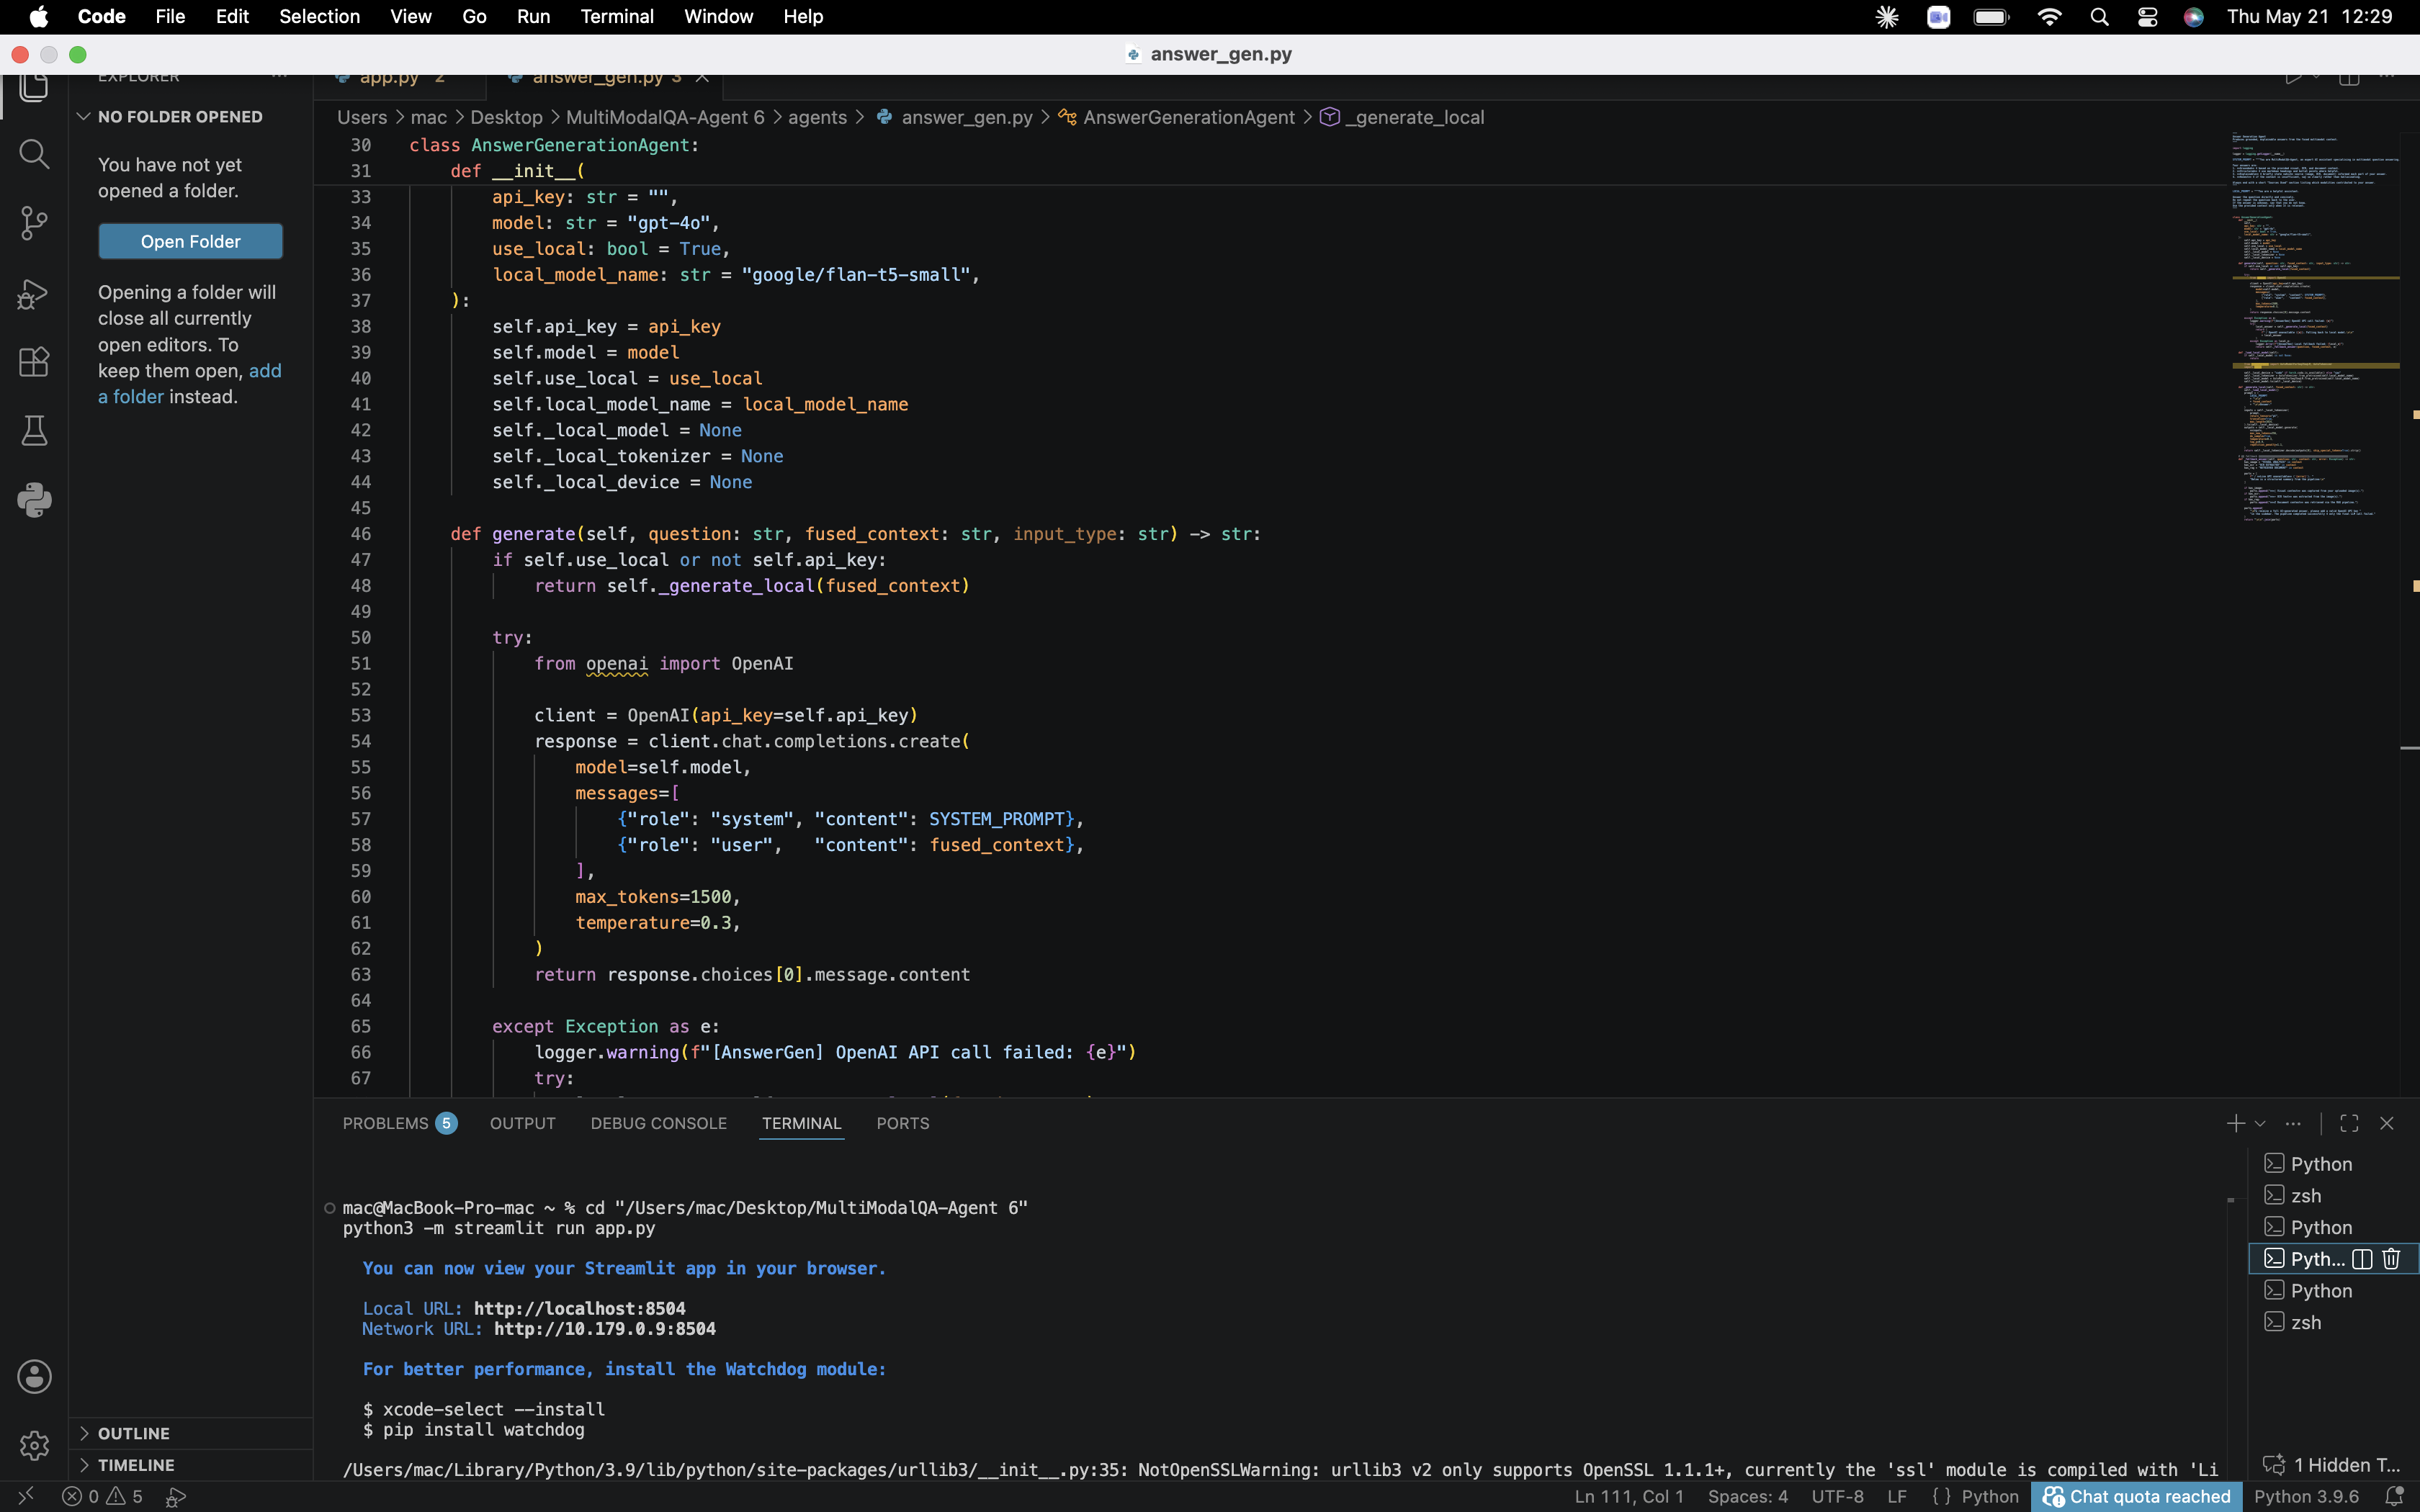
\includegraphics[width=0.48\textwidth]{code_screenshot.png}
\caption{Python codebase implementation for the Answer Generation Agent.}
\label{fig:code_screenshot}
\end{figure}

Fig. \ref{fig:app_screenshot} highlights the live web-based application interface built using Streamlit and accessed locally. The UI is split into a system configuration sidebar (which coordinates key management, local vs. cloud API routing, OCR controls, and vector RAG activation) and a primary agent conversation window with visual upload dropzones and dynamic pipeline status trackers.

\begin{figure}[htbp]
\centering
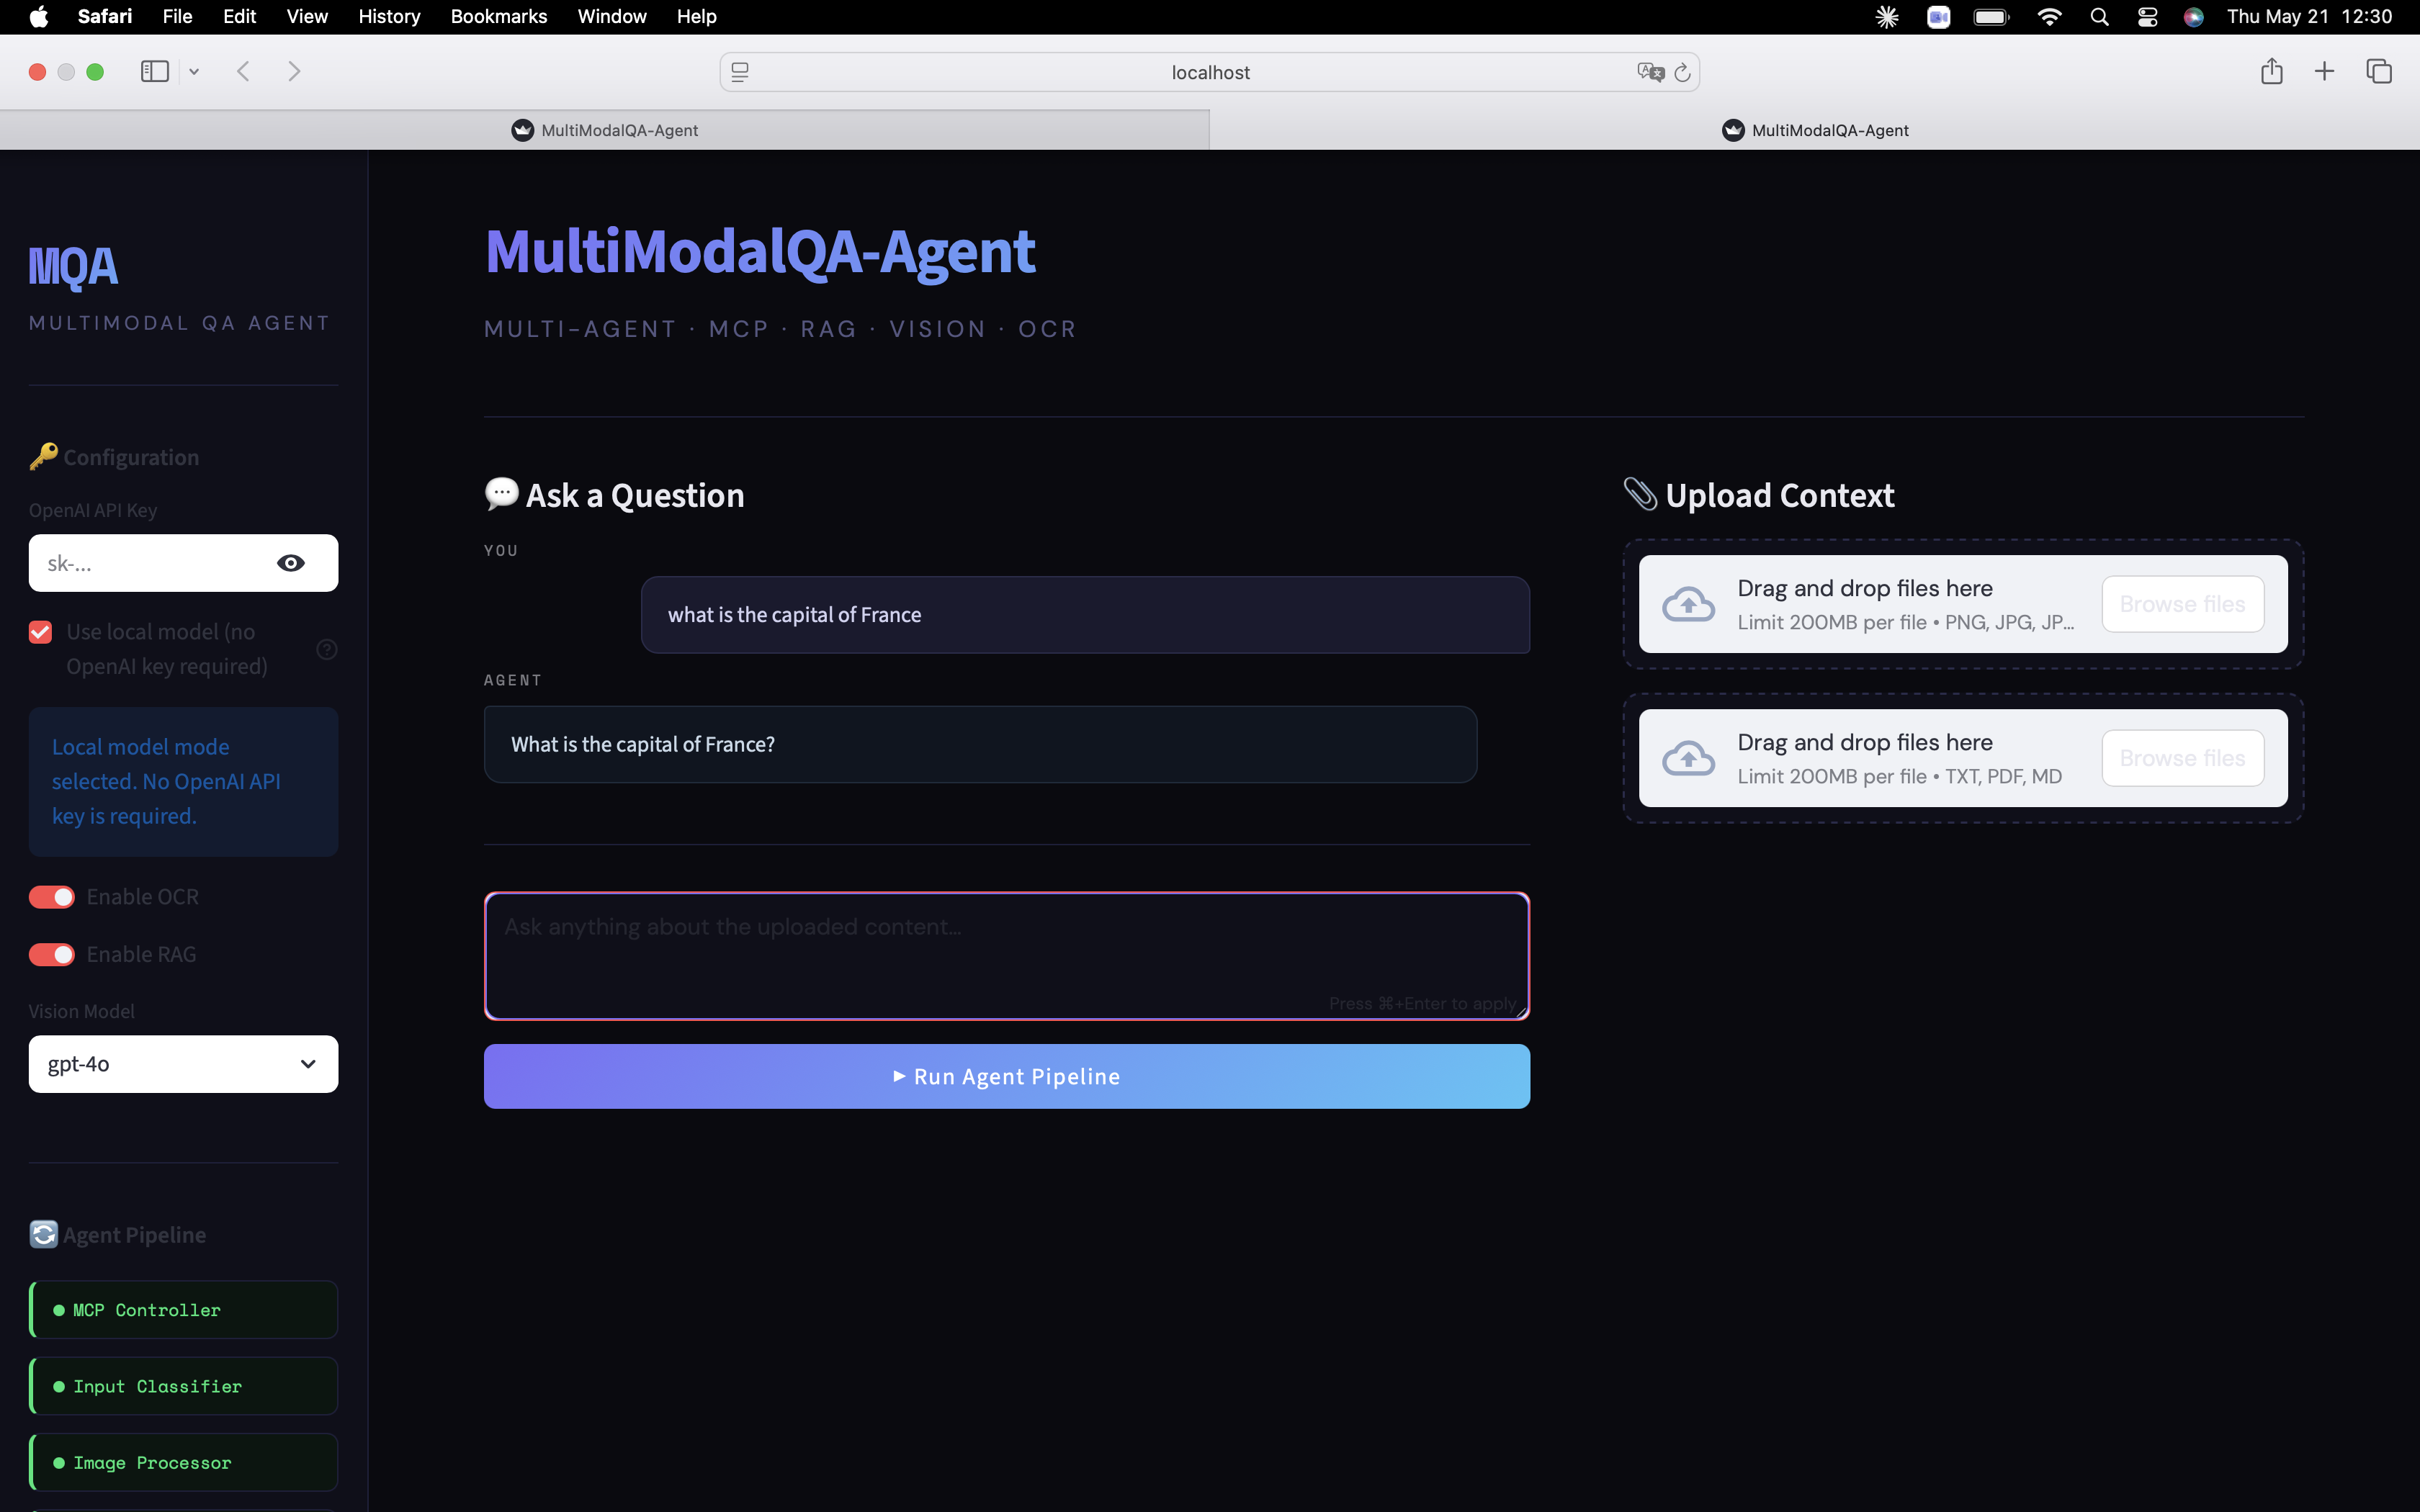
\includegraphics[width=0.48\textwidth]{app_screenshot.png}
\caption{Live Streamlit user interface demonstrating multimodal query processing.}
\label{fig:app_screenshot}
\end{figure}

\begin{thebibliography}{00}
\bibitem{b1} A. Radford et al., ``Learning Transferable Visual Models From Natural Language Supervision,'' \textit{Proceedings of the International Conference on Machine Learning (ICML)}, 2021.
\bibitem{b2} P. Lewis et al., ``Retrieval-Augmented Generation for Knowledge-Intensive NLP Tasks,'' \textit{Advances in Neural Information Processing Systems (NeurIPS)}, vol. 33, pp. 9459--9474, 2020.
\bibitem{b3} S. Yao et al., ``ReAct: Synergizing Reasoning and Acting in Language Models,'' \textit{International Conference on Learning Representations (ICLR)}, 2023.
\bibitem{b4} W. Wu et al., ``AutoGen: Enabling Next-Gen LLM Applications via Multi-Agent Conversation,'' \textit{arXiv preprint arXiv:2308.08155}, 2023.
\bibitem{b5} J. Devlin, M. Chang, K. Lee, and K. Toutanova, ``BERT: Pre-training of Deep Bidirectional Transformers for Language Understanding,'' \textit{Proceedings of NAACL-HLT}, pp. 4171--4186, 2019.
\bibitem{b6} T. Brown et al., ``Language Models are Few-Shot Learners,'' \textit{Advances in Neural Information Processing Systems (NeurIPS)}, vol. 33, pp. 1877--1901, 2020.
\bibitem{b7} A. Vaswani et al., ``Attention Is All You Need,'' \textit{Advances in Neural Information Processing Systems (NeurIPS)}, 2017.
\bibitem{b8} OpenAI, ``GPT-4 Technical Report,'' 2023.
\bibitem{b9} A. Jaegle et al., ``Perceiver IO: A General Architecture for Structured Inputs and Outputs,'' \textit{International Conference on Machine Learning (ICML)}, 2021.
\bibitem{b10} K. He, X. Zhang, S. Ren, and J. Sun, ``Deep Residual Learning for Image Recognition,'' \textit{Proceedings of the IEEE Conference on Computer Vision and Pattern Recognition (CVPR)}, 2016.
\bibitem{b11} P. Odimmegwa, T. L. Muparutsa, H. Dyabi, and E. Arapbaev, ``MultiModalQA-Agent Codebase Repository,'' GitHub, 2026. [Online]. Available: \url{https://github.com/Paul1812/MultiModalQA-Agent}
\end{thebibliography}
\end{document}
